\chapter{Análisis comparativo}
Android e iOS son dos plataformas muy populares entre los dispositivos móviles. Es por ello, que existes muchas  muchas formas de comparar sus respectivos módulos de seguridad.\\
La medida de comparación propuesta en \cite{YA2014} consiste en analizar la seguridad de una aplicación móvil en cada fase del ciclo de vida, comparándola en cada plataforma.\\
En \cite{HYGZD2013} el enfoque es distinto. Se centra en comparar los permisos requeridos a cada plataforma al momento de instalar por aplicaciónes presentes en ambas plataformas.\\
En \cite{Gor16, BCLR15, Rom14} el enfoque propuesto es distinto. El objetivo que persiguen es desarrollar una especificacion formal que describa el modulo de seguridad de Android.\\
En este capítulo se propone una forma de comparar distinta a las anteriores. Consiste en analizar cuales permisos se pueden modificar en tiempo de ejecución.\\
\section{Analizando Android}
Debido a que cada aplicación Android opera en un entorno aislado\footnote{Ver seccion \nameref{ch01-sandbox}.}, las aplicaciones deben compartir de manera explícita recursos y datos. El camino utilizado para realizar dicho intercambio es la declaración de permisos, tal como se introdujo en la sección \ref{ch01-permisos}.\\
En las versiones anteriores a Android Marshmallow, al prepararse para instalar una aplicación, el sistema mostraba un diálogo al usuario indicando los permisos solicitados y se le solicitaba si deseaba continuar con la instalación. En caso afirmativo, el sistema otorgaba todos los permisos solicitados. El usuario no podía otorgar o denegar permisos individuales; debía otorgar o denegar todos los permisos solicitados como un bloque. Una vez concedidos, los permisos se aplicaban mientras la aplicación estaba instalada. Solo se eliminaban si se desinstala una aplicación, por lo que una posterior reinstalación dará como resultado la visualización de permisos.\\
\begin{figure}[hbtp]
    \centering
    \begin{subfigure}{0.3\linewidth}
        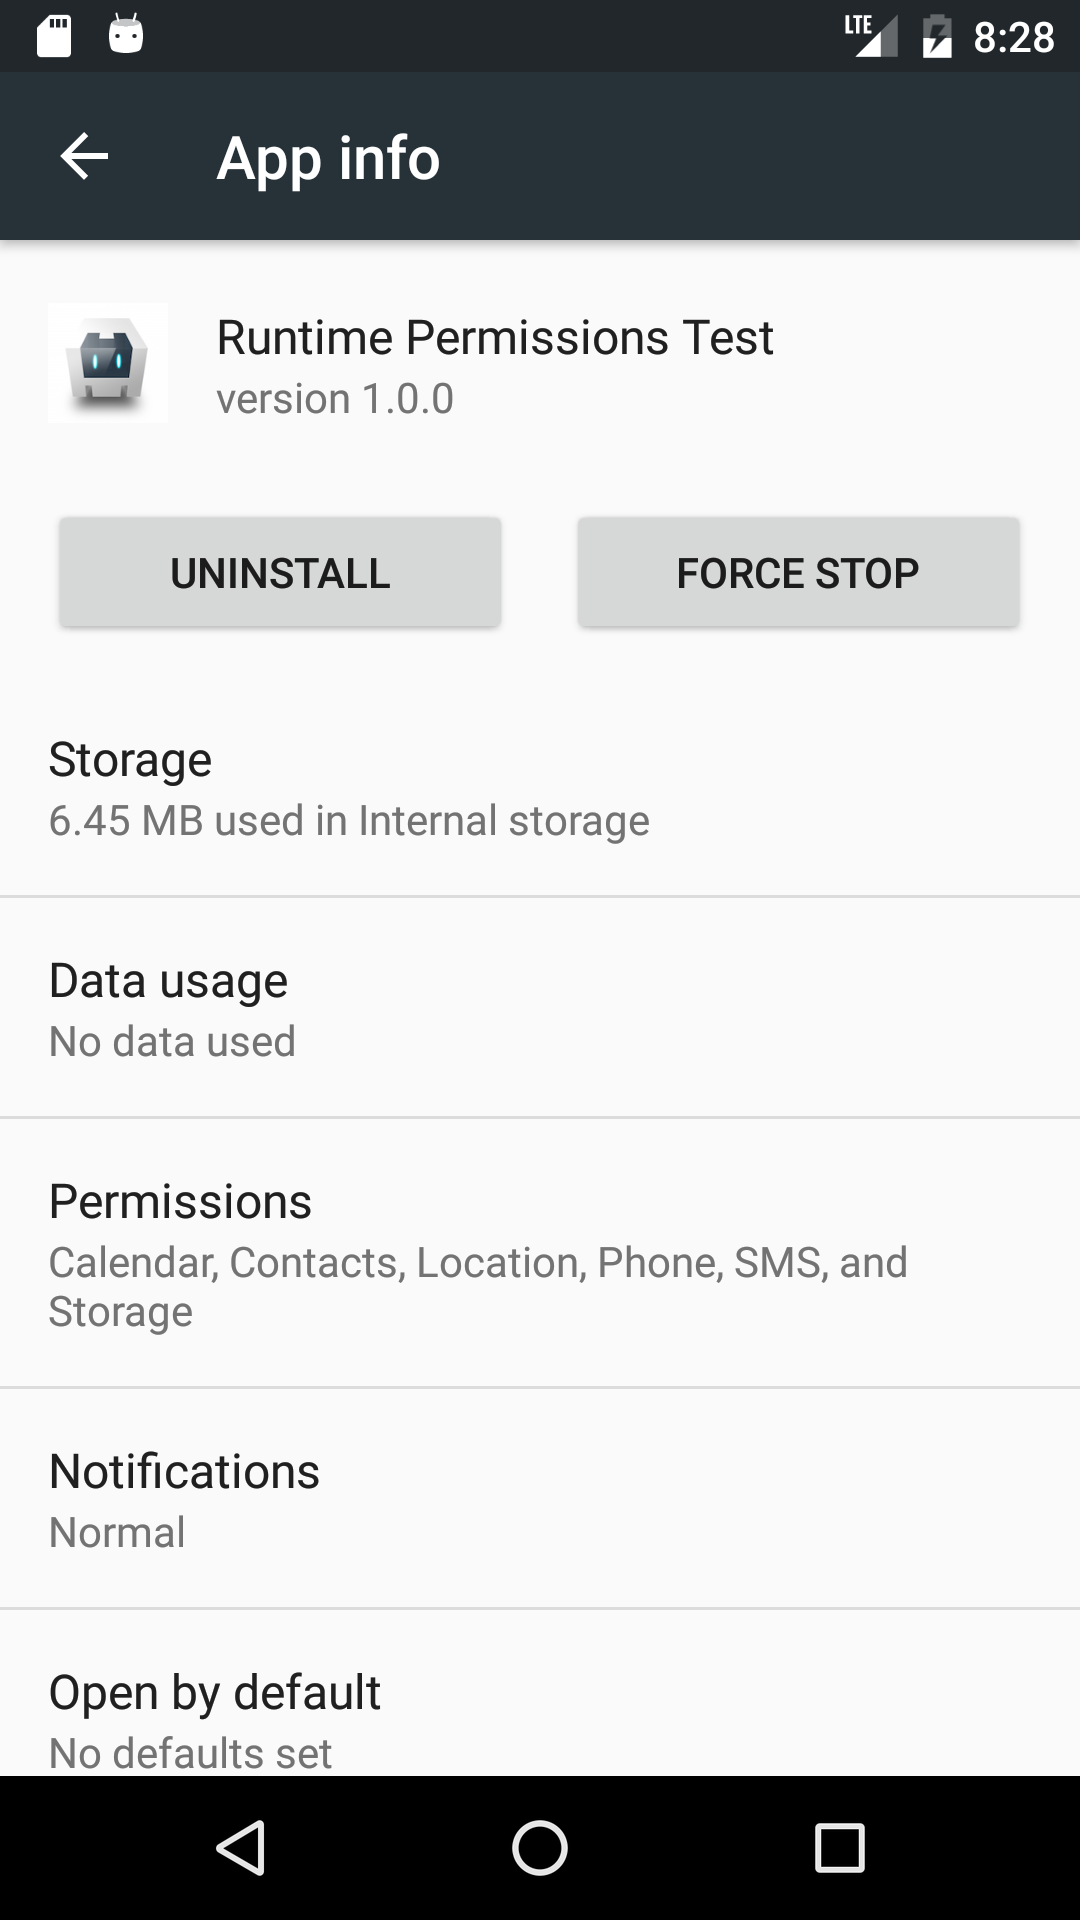
\includegraphics[width=\linewidth]{imgs/chapter1/app-info}
    \end{subfigure}
    \begin{subfigure}{0.3\linewidth}
        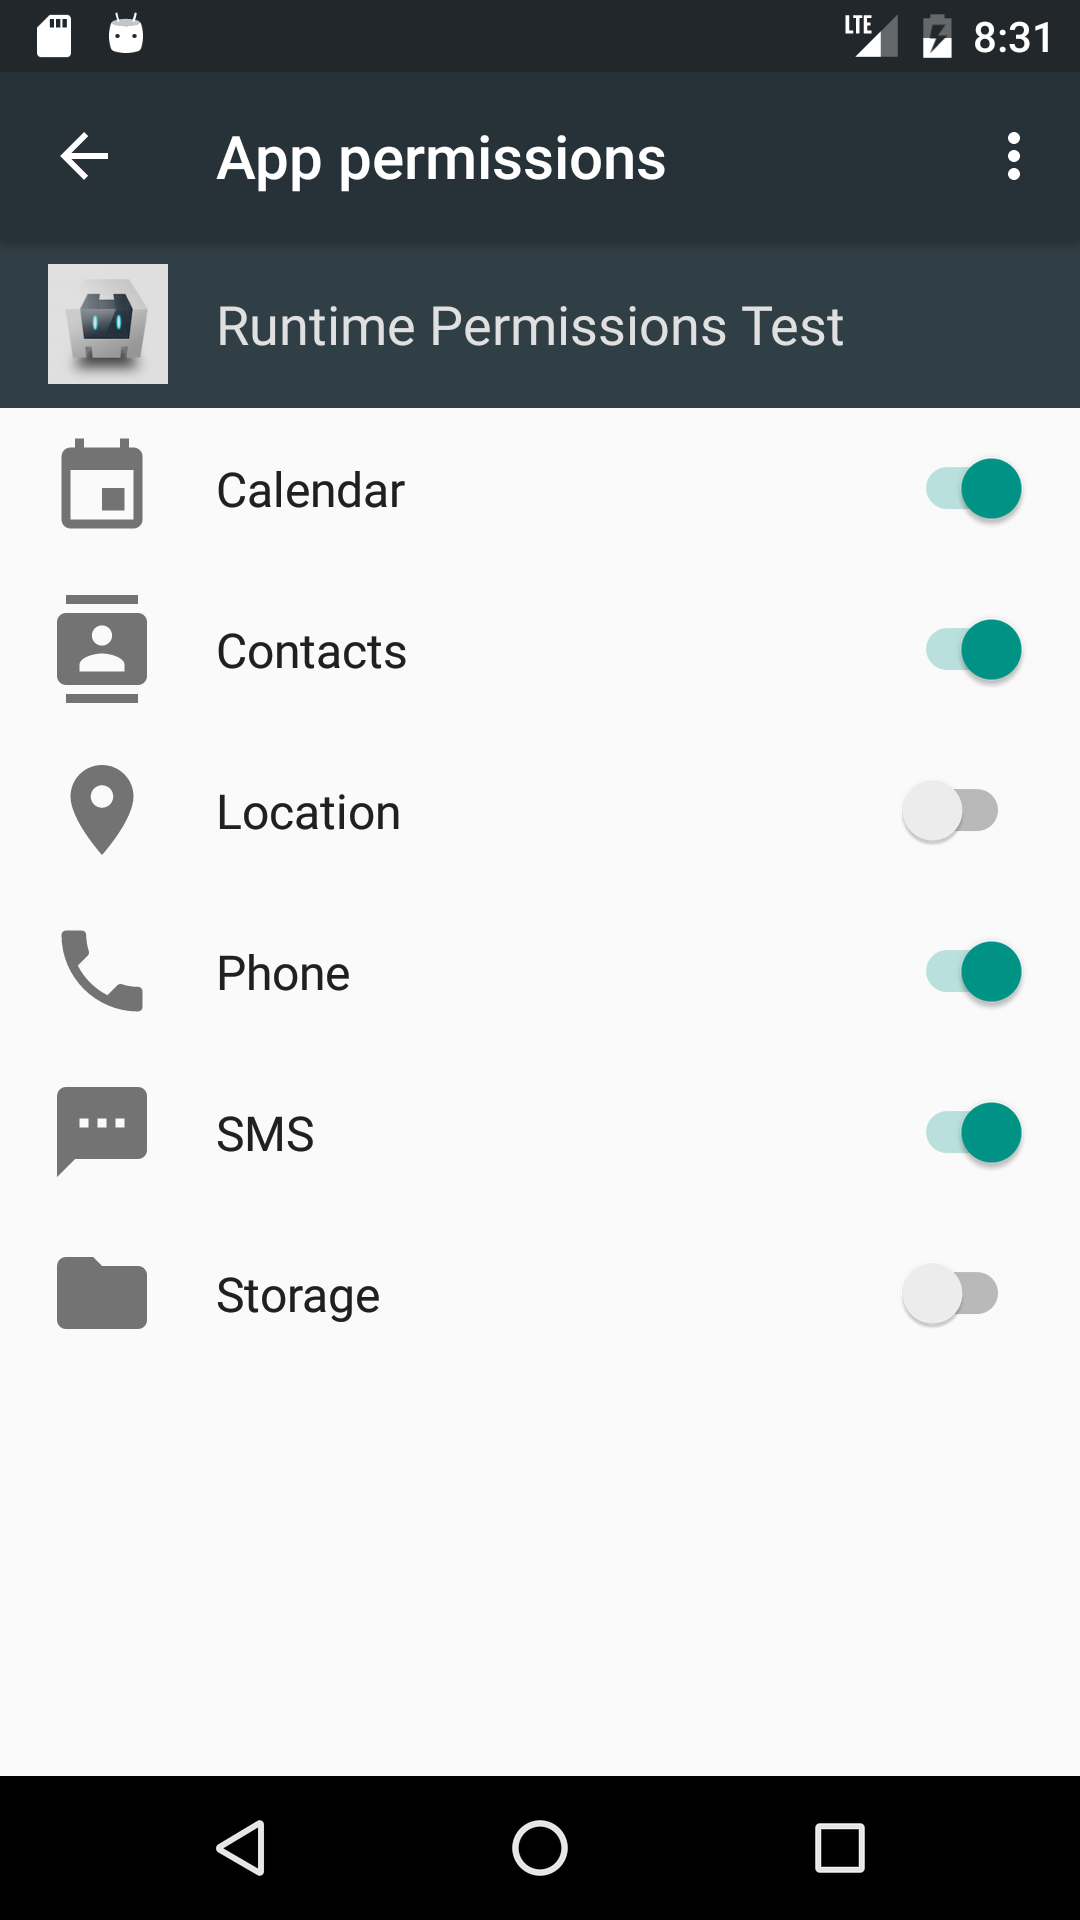
\includegraphics[width=\linewidth]{imgs/chapter1/app-permissions}
    \end{subfigure}
    \caption{Descripción general de los permisos otorgados.}
	\label{fig:ch01:app-permissions-overview}
\end{figure}
A partir de la versión 6.0 se propone un nuevo modelo de permisos, donde los usuarios pueden administrar los permisos de una aplicación en tiempo de ejecución, ganando una mejor visibilidad y un mejor control, como se observa en la Figura \ref{fig:ch01:app-permissions-overview}. En este modelo, los permisos se agrupan para facilitar el control privacidad de los usuarios de aplicaciones. Dichos grupos son:
\begin{itemize}
    \item \emph{Almacenamiento:} Regula el acceso al almacenamiento externo \footnote{En Android, cuando se habla de almancenamiento externo, se refiere a la tarjeta SD.}, permitiendo la lectura o la escritura desde el mismo.
    \item \emph{Calendario:} Permiten leer, modificar o eliminar los datos del calendario del usuario.
    \item \emph{Cámara:} Regula el acceso de la cámara del dispositivo para capturar imágenes y/o videos.
    \item \emph{Contactos:} Permiten leer, modificar o eliminar los contactos almacenados en el dispositivo.
    \item \emph{Localización:} Regula el acceso a la ubicación del dispositivo, ya sea la ubicación precisa (GPS) o la aproximada (WIFI/Móvil).
    \item \emph{Mensajes SMS:} Permite a una aplicación obtener todos los permisos relacionados a los SMS, tales como leer, escribir, enviar, etc.
    \item \emph{Micrófono:} Regula el acceso al micrófono del dispositivo, permitiendo además grabar el sonido obtenido. No se incluyen en este grupo los permisos para capturar sonidos provenientes de una llamada telefónica.
    \item \emph{Teléfono:} Permite a una aplicación obtener todos los permisos relacionados a la telefonía, tales como iniciar una llamada, manipular el log de llamadas, obtener datos de una llamada en curso, etc.
    \item \emph{Sensores:} Permite acceder a los datos de los sensores que el usuario utiliza para medir lo que esta sucediendo en su cuerpo, tales como el ritmo cardíaco.
\end{itemize}
Por otra parte, a las aplicaciones no se les conceden los permisos durante la instalación ya que el nuevo modelo de obliga todas las aplicaciones solicitarlos en tiempo de ejecución, como se observa en la Figura \ref{fig:ch01:permission-request}. Ya que el usuario puede revocar los permisos en cualquier momento, una aplicación necesita comprobar si dispone de los permisos cada vez que se ejecuta.
\begin{figure}[hbtp]
    \centering
    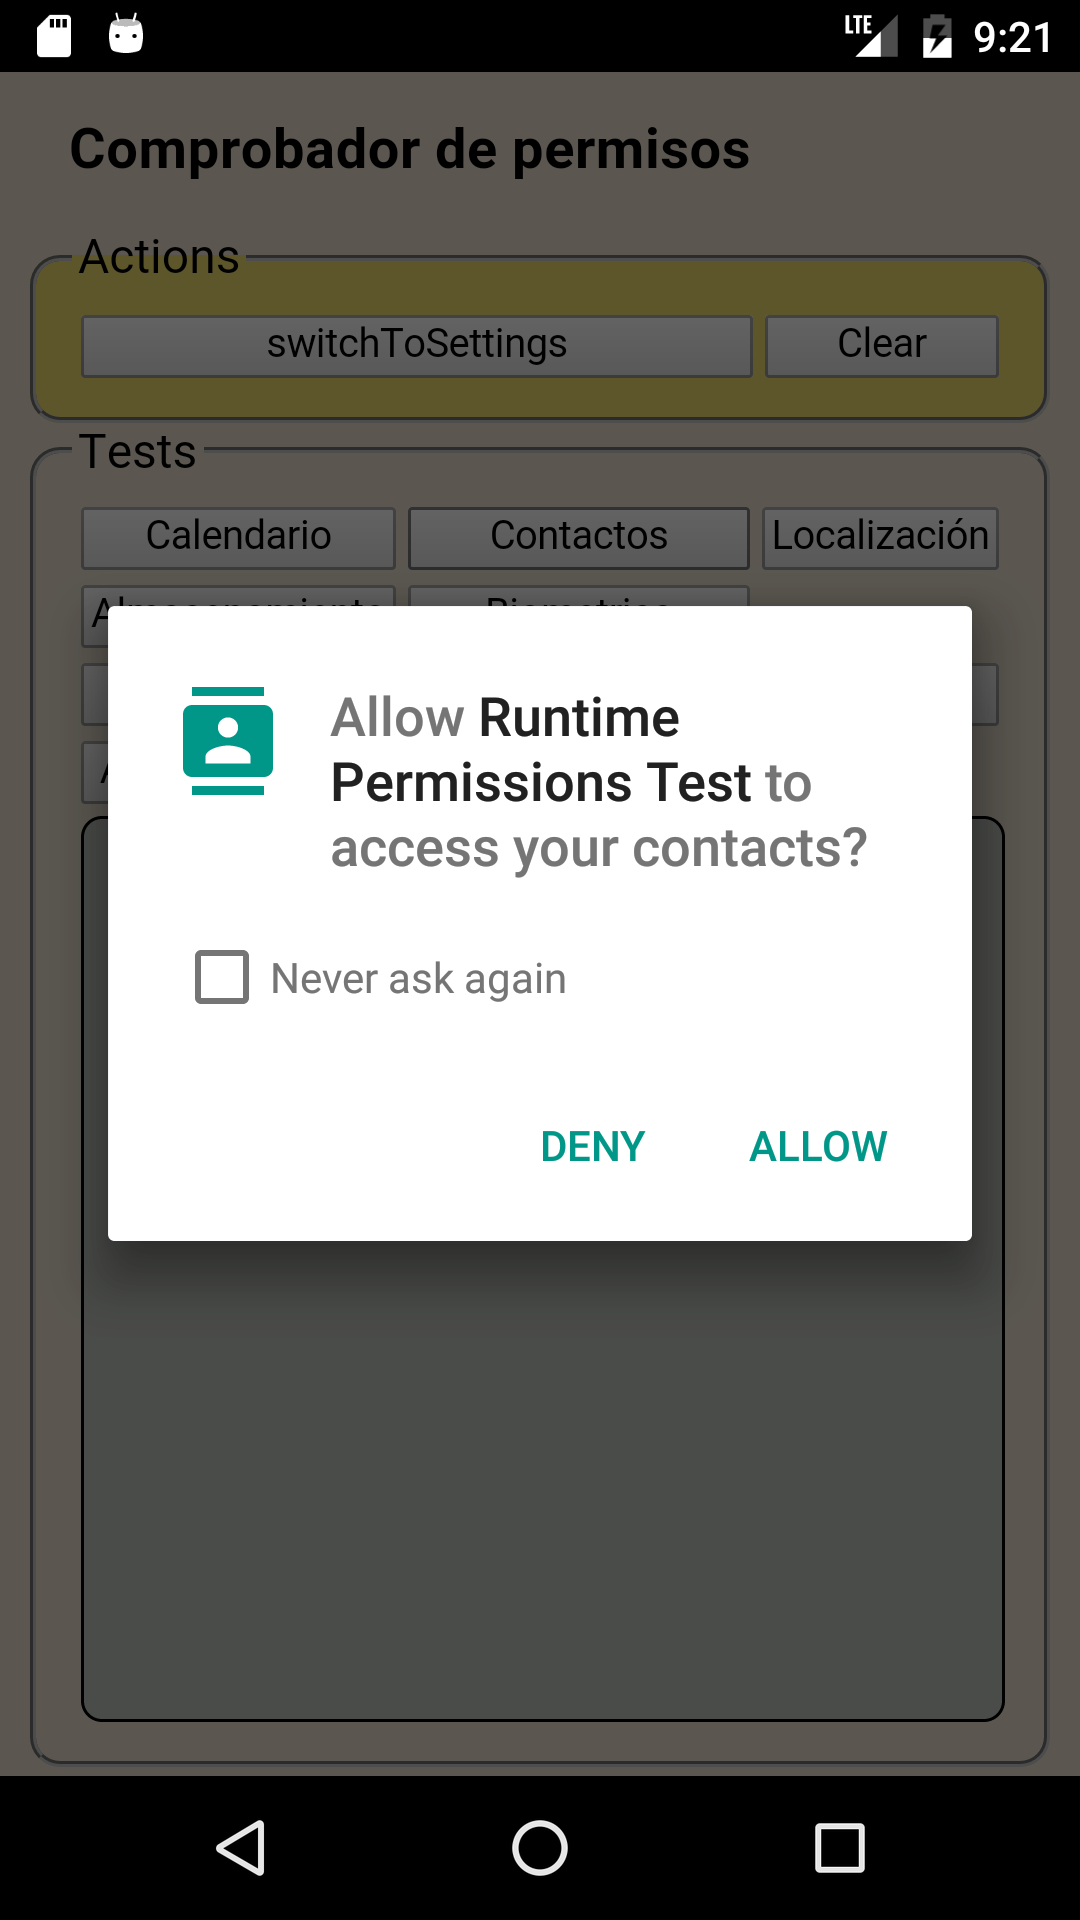
\includegraphics[width=0.3\linewidth]{imgs/chapter5/allow_contact}
    \caption{Ejemplo de solicitud de un permiso en tiempo de ejecución.}
    \label{fig:ch01:permission-request}
\end{figure}
\subsection*{Detalle de los tests}
Luego de instalar la aplicación, se observa que la misma no tiene ningún permiso:
\begin{figure}[!ht]
	\centering
	\begin{subfigure}{.32\textwidth}
		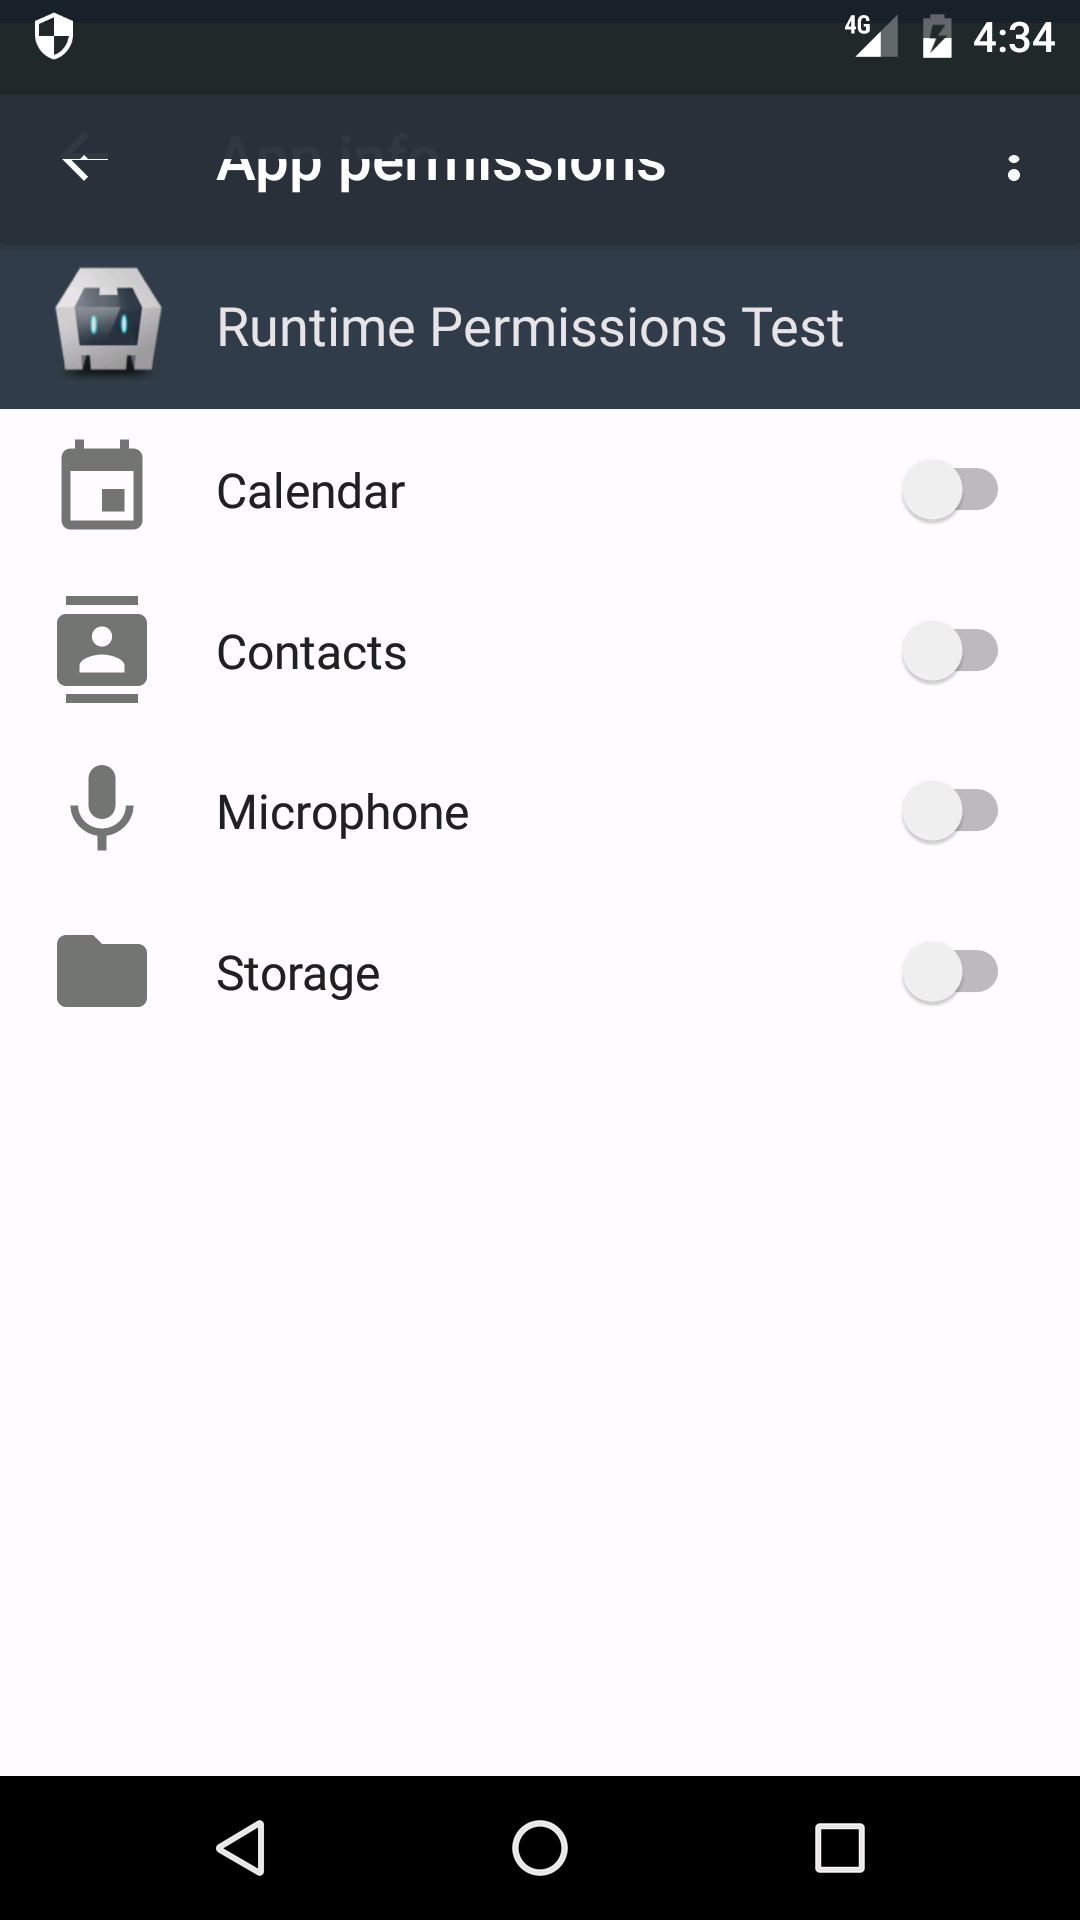
\includegraphics[width=4cm]{chapter5/without_permissions}
		\caption{\textit{Runtime Permissions Test} no tiene ningún permiso $peligroso$}
		\label{fig:chapter05:without_permissions}
	\end{subfigure}
	\begin{subfigure}{.32\textwidth}
		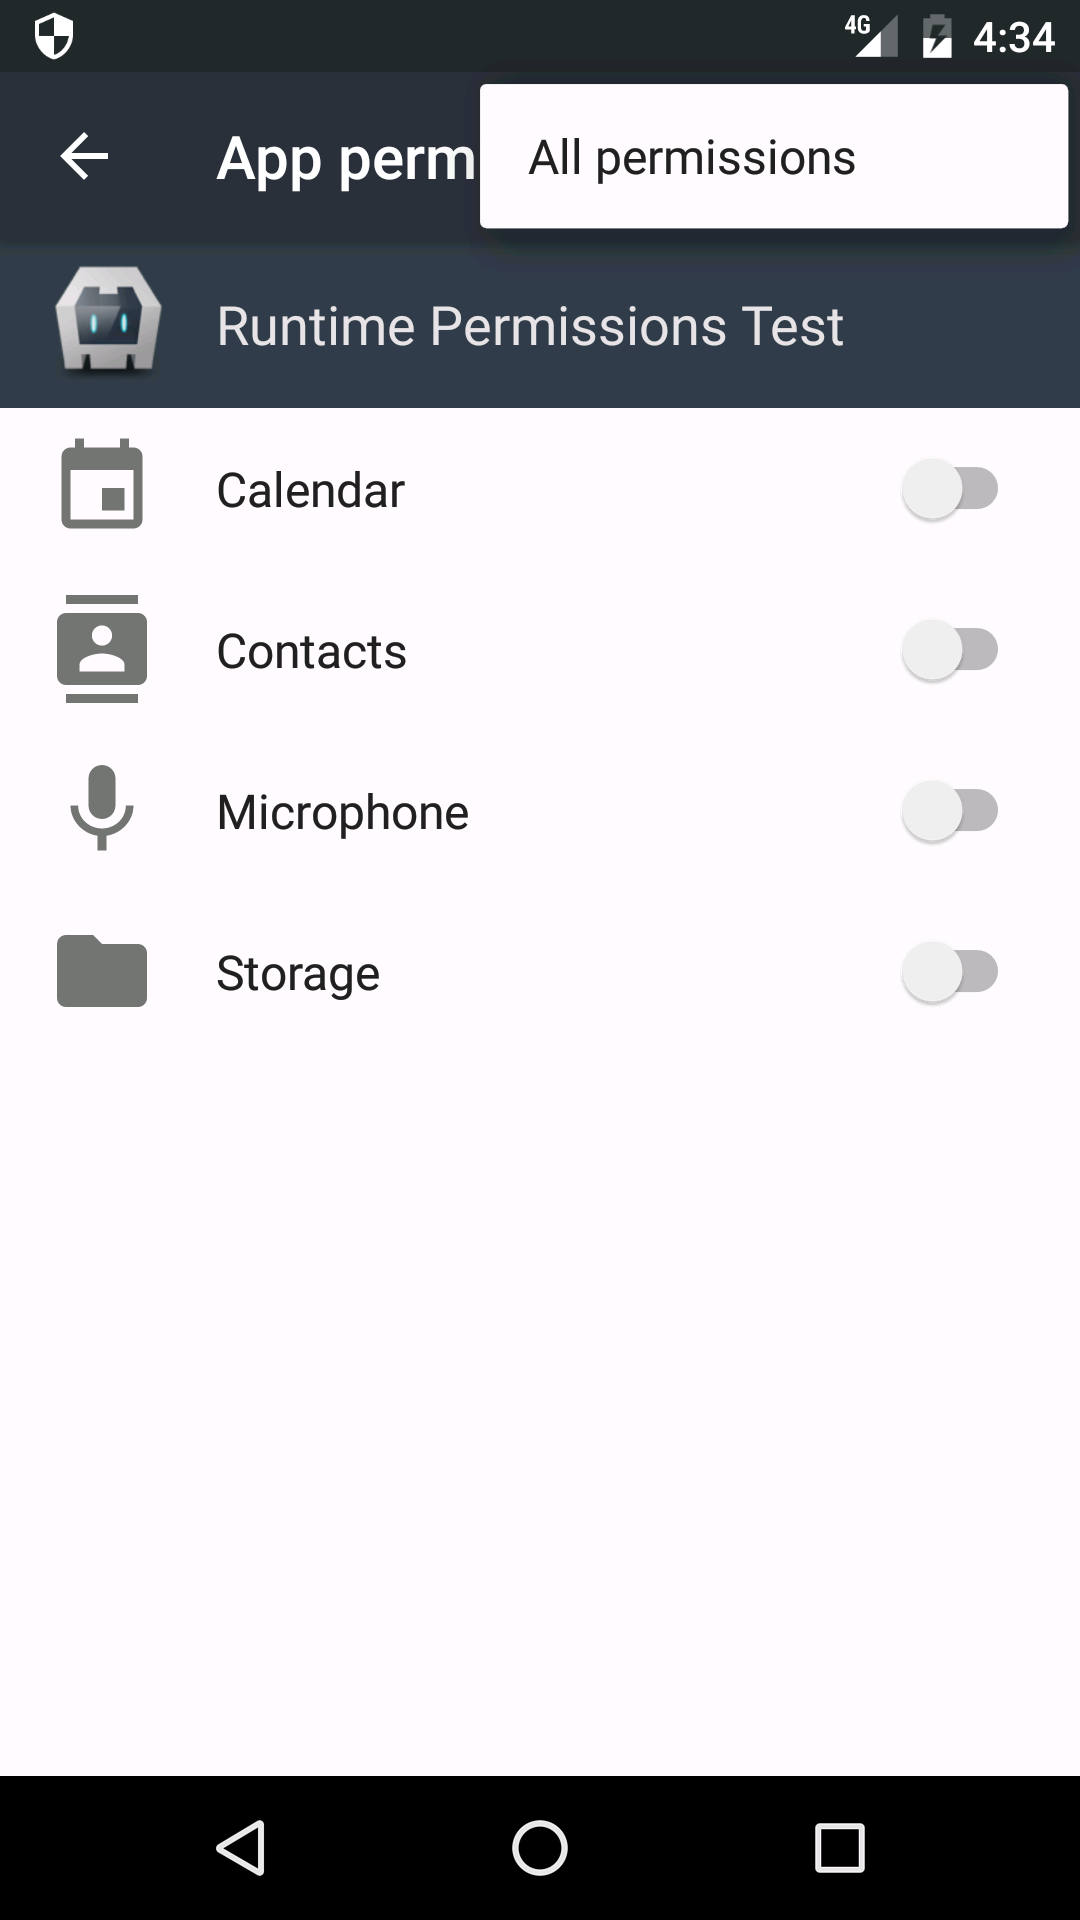
\includegraphics[width=4cm]{chapter5/all_permissions}
		\caption{Si se presiona sobre los tres puntos, se acceden a todos los permisos}
		\label{fig:chapter05:all_permissions}
	\end{subfigure}
	\begin{subfigure}{.32\textwidth}
		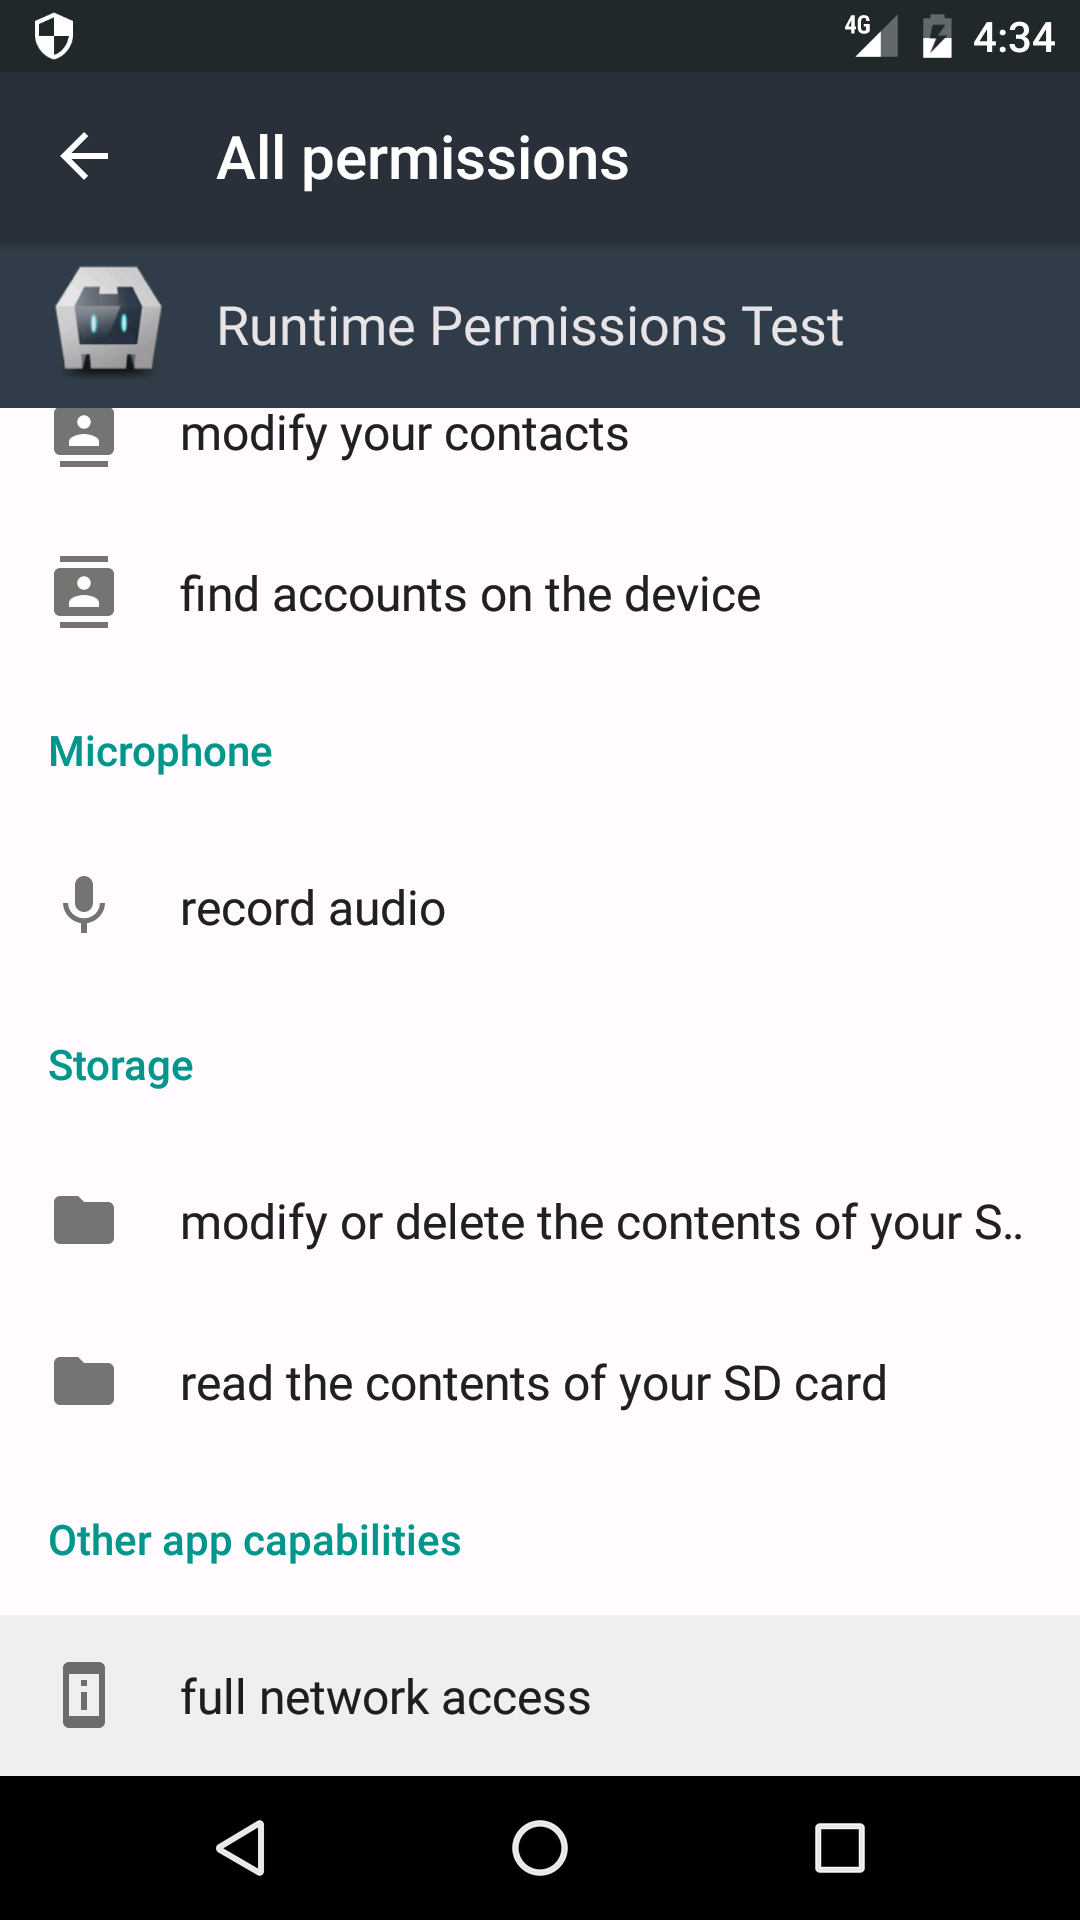
\includegraphics[width=4cm]{chapter5/always_have_internet}
		\caption{\textit{Runtime Permissions Test} tiene todos los permisos $normales$}
		\label{fig:chapter05:always_have_internet}
	\end{subfigure}
	\caption{\textit{Android App Permissions, API\textgreater 23}}
	\label{fig:chapter05:android_permissions}
\end{figure}\\
Sin embargo, si se muestran todos los permisos de la aplicación, notará que se tienen todos los permisos $normales$ que requiera. Por ejemplo, en la Figura \ref{fig:chapter05:always_have_internet} se observa que tenemos permiso de acceso a internet.
    

\newpage

\section*{Analizando iOS}
Los controles de privacidad en iOS dan el control sobre qué aplicaciones tienen acceso a la información almacenada en su dispositivo iOS. Su enfoque es distinto ya que focaliza en componentes del sistema, permitiendo al usuario denegar (o permitir) el acceso de una aplicación a un determinado componente. El usuario puede modificar la configuración de privacidad en $Ajustes > Privacidad$. En ella se encuentra una lista de componentes, como se observa en la figura \ref{fig:chapter03:iospermCapture}. Para cada uno de ellos, figuran las aplicaciones que pidieron permiso para usar dicho componente. Se pueden agregar o quitar el permiso de cualquier aplicación que ha solicitado el acceso a los datos. Cabe aclarar que una aplicación puede utilizar sus datos sólo si se le ha dado permiso.\\

\begin{figure}[!pb]
	\begin{subfigure}{.4\textwidth}
		\centering
		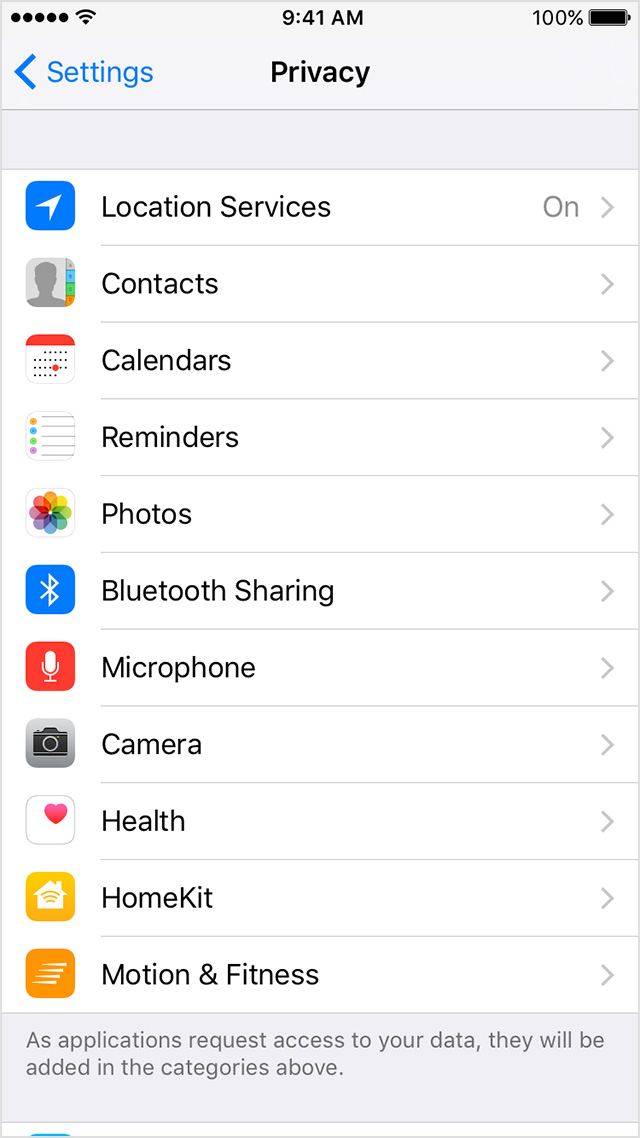
\includegraphics[width=135px]{chapter3/iphone6-ios9-settings-privacy}
    		\caption{iOS 9.3}
   		\label{fig:chapter03:iospermCapture}
	\end{subfigure}
	\begin{subfigure}{.55\textwidth}
	    \centering	
		\begin{tabular}{|c|c|}
			\hline
			\rowcolor{gray!50}
			Permissions		 					& Subgroup\\ \hline
			\multirow{12}{*}{LOCATION SERVICES} 	& Cell Network Search \\
								 				& Compass Calibration \\
												& Find My iPhone \\
												& HomeKit \\
												& Location-Based Alerts \\
												& Location-Based iAds \\
												& Motion Calibration \& Distance \\
												& Safari \& Spotlight Suggestions \\
												& Settings Time Zone\\
												& Share My Location \\
												& Wi-Fi Networking \\
												& Frequent Locations \\ \hline
			Contacts				& \\ \hline
			Calendars			& \\ \hline
			Reminders			& \\ \hline
			Photos				& \\ \hline
			Bluetooth Sharing 	& \\ \hline
			Microphone 			& \\ \hline
			Camera 				& \\ \hline
			Health 				& \\ \hline
			HomeKit 				& \\ \hline
			Social Media Accounts& \\ \hline
			Diagnostics \& Usage	& \\ \hline		
			Advertising			& \\ \hline
		\end{tabular}
		\caption{Permisos modificables por el Administrador de Privacidad de iOS}
		\label{tab:chapter03:iosperm}
	\end{subfigure}
\end{figure}
La lista mencionada anteriormente contiene algunos componentes cuyo nombre es lo suficientemente descriptivo como para saber que estamos permitiendo o denegando. A continuación se hará una breve descripción sobre los componentes de la lista:
\begin{itemize}
	\item \textbf{Location Services:} permite a las aplicaciones y/o a las páginas web determinar aproximadamente su ubicación. Dependiendo de su dispositivo y de los servicios disponibles, se utiliza una combinación de cierta información del celular, Wi-Fi, Bluetooth y GPS para determinar su ubicación.
	\item \textbf{Contacts:} permite a las aplicaciones el acceso a los contactos.
	\item \textbf{Calendars:} regula el acceso a los calendarios, incluyendo las citas y eventos incluidos en él.
	\item \textbf{Reminders:} permite a las aplicaciones la lectura y/o escritura de los recordatorios.
	\item \textbf{Photos:} permite a una aplicación el acceso a las fotos y al álbum de cámara directamente, ya sea para subir nuevas imágenes a un servicio desde el dispositivo iOS, o para guardar nuevas imágenes a la aplicación Fotos. También pueden tener la capacidad de crear un álbum de fotos dentro de la aplicación de fotos.
	\item \textbf{Bluetooth Sharing:} permite controlar cuáles aplicaciones pueden compartir datos a través de Bluetooth.
	\item \textbf{Microphone:} regula el acceso al micrófono.
	\item \textbf{Camera:} regula el acceso al la cámara del dispositivo.
	\item \textbf{Health:} permite a las aplicaciones conocer la información de su salud y estado físico, tanto las cargadas como las que recopiló el dispositivo.
	\item \textbf{HomeKit:} regula el acceso a los accesorios hogareños registrados en el dispositivo.			
	\item \textbf{Social Media Accounts:} permite a las aplicaciones realizar actividades relacionadas a una red social, tales como crear una sesión de red, obtener el feed de actividad para un usuario, hacer una nueva entrada. También permite publicar una entrada a un canal de actividades o realizar ajustes de las propiedades de una publicación, añadir archivos adjuntos, etc.
	\item \textbf{Diagnostics \& Usage:} regula cuáles datos de diagnóstico sobre el dispositivo se envían a Apple. Esos datos incluyen información sobre el rendimiento del sistema, capacidad restante en el dispositivo, detalles acerca de sus especificaciones del dispositivo y del sistema operativo, entre otras.
	\item \textbf{Advertising:} permite inhabilitar los anuncios basados en intereses.
\end{itemize}
\newpage

\section*{Resultados}
Al momento de realizar el análisis, se tuvieron en cuenta las coincidencias y las diferencias entre ambas plataformas.\\
Entre las primeras, podemos mencionar que las dos tienen dispositivos en común a los cuáles se les pueden modificar permisos en \textit{runtime}: micrófono, cámara, GPS, y sensores biométricos. También se aplican dichos permisos a componentes que contienen información sensible del usuario, tales como el calendario, los contactos y las fotos.\\
Entre las segundas, podemos mencionar permisos que tiene uno pero no el otro. Por ejemplo, Android tiene la permisos sobre el almacenamiento externo. Este permiso no tiene sentido en iOS, ya que los iPhone solamente tienen almacenamiento interno. iOS, por su parte, tiene integrado el manejo de ciertos dispositivos hogareños. También dispone de un servicio tracking de publicidad, el cual permite recomendaciones sobre los gustos del usuario. Por ello, agrega permisos para dichos componentes, los cuales no existes como componentes en Android.\\
Como consecuencia de lo mencionado anteriormente, se encontraron permisos que son comparables entre sí y otros que no lo son. Cabe aclarar que ciertos permisos se agruparon. Por ejemplo, en Android, los recordatorios forman parte del calendario; mientras que en iOS están separados. Los resultados se volcaron en la tabla \ref{tab:chapter03:compPerm}.\\

\begin{table}[!ht]
	\center
	\begin{tabular}{|c|c|c|}
		\hline
		\rowcolor{gray!50}
		\multicolumn{3}{|c|}{Permissions} \\					\hline
		\rowcolor{gray!50}
		Commons 	& Only Android	& Only iOS \\				\hline
		Calendar\&Events	& -		& -	\\						\hline
		Contacts	& -				& - \\						\hline
		Camera		& -				& -	\\						\hline
		Location	& -				& -	\\						\hline
		-			& -				& Bluetooth Sharing \\		\hline
		Microphone  & -				& - \\						\hline
		-			& Phone			& -	\\						\hline
		Body Sensors	& -			& - \\						\hline
		-			& SMS			& - \\						\hline
		-			& Storage		& - \\						\hline
		-			& -				& Homekit \\				\hline
		-			& -				& Social Media Accounts \\	\hline
		-			& -				& Diagnostic \& Usage \\	\hline		
		-			& -				& Advertising \\			\hline
	\end{tabular}
	\caption{Comparación de permisos entre Android 6.0 e iOS}
	\label{tab:chapter03:compPerm}
\end{table}
Para finalizar el capítulo, se mencionan las conclusiones que se encontraron.\\
Es importante destacar la falta de granularidad en algunos aspectos. Android no toma como permiso peligroso los datos de las redes sociales. Tampoco el permiso para compartir cosas por Bluetooth. Por otro lado, iOS no tiene la suficiente granularidad para administrar el acceso a las llamadas telefónicas, su historial, etc. Tampoco contempla los datos móviles ni los SMS. En estos casos, el permiso es a nivel de teléfono y no a nivel de aplicación.\\

Otra cosa a destacar es que en Android el permiso es a nivel de grupo. Cuando se requiere que el usuario permita cierto permiso para una aplicación, lo que sucede es que la aplicación obtiene todos los permisos del grupo. Por ejemplo, si se pide permisos del grupo "Calendario" se obtienen los permisos tanto para leer y para escribir. Para el caso del calendario puede llegar a ser razonable tener los dos permisos pero para otros casos no lo es. Como consecuencia de ello, el usuario esta delegando a una aplicación demasiados permisos.\\